We prototype our models in an FPGA-Accelerated simulation framework that builds on
the Rocket-Chip \cite{rocketchip} infrastructure (similar to
\cite{strober}). Our designs are developed in Chisel, a high-level
hardware-description language written in Scala. Building on this infrastructure
allows us to leverage a large amount of available open-source IP and a growing
software ecosystem that includes GCC, Linux and LLVM.

Our framework makes use of FIRRTL~\cite{firrtl}, an intermediate representation
(IR) for RTL that has frontends for both Chisel and Verilog, and can target
both FPGA and ASIC flows by emitting optimized Verilog output. FIRRTL enables
the implementation of compiler passes on top its IR framework. These passes
can, for example, apply FPGA-optimizations, add instrumentation, and
automatically produce scan chains for debugging and power
estimation\cite{strober} -- all without requiring modifications to the source
RTL.

\begin{figure}
	\centering
	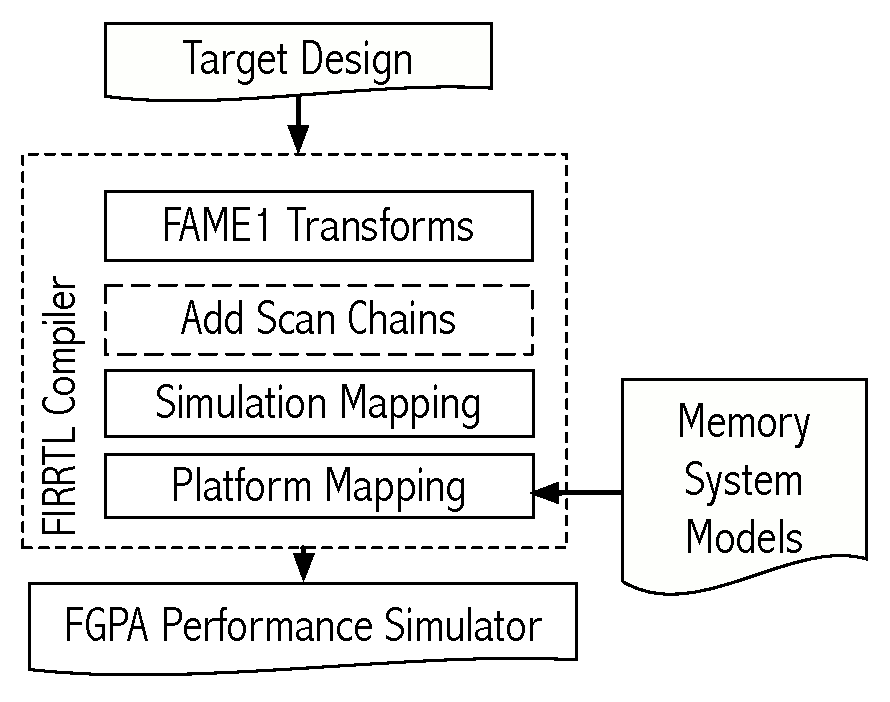
\includegraphics[width=7cm]{figures/firrtl.pdf}
	\caption{FIRRTL custom transforms for the FPGA simulator}
	\label{fig:firrtl}
\end{figure}


\section{Host-Target Decoupling in MIDAS}

\section{Transformations of Source RTL}

MIDAS uses FIRRTL compiler passes to preform transformation source RTL into
host-decoupled models. The most important of these is the FAME-1
transformation, which adds to requsite logic to host-decouple target RTL, so
that it may conform to a RAMP model of execution. \TODO{See Section}. In figure
\TODO{Auto-transformation} below, the procedure through which source RTL is
host decoupled is illustated.


Additional transformations may be invoked to add scan
chains and I/O trace buffers for debugging, and for state snapshotting for use
with Strober\cite{strober}.

\section{Platform Mapping}

\section{Target Machines}

While this approach is applicable to arbitrary RTL, one challenge lies in
sourcing the RTL to build a realistic target. While we build on RocketChip and
\RISCV, our approach could in principle be used with other open-source designs
such as OpenPiton\cite{openpiton} and FabScalar\cite{fabscalar}.
